\textcolor{secundario}{ENFOQUE RESIDUAL DIN\'AMICO}. Una vez estimado el valor del capital invertido total del negocio, al perito valuador de negocios le corresponde identificar el activo tangible total de la firma a valor de mercado, para poder as\'i aplicar un razonamiento residual que permite determinar el valor de mercado del activo intangible (\autoref{fig:def_act_int}), seg\'un el principio econ\'omico mencionado en la \autoref{fig:valor_firma}.

\begin{figure}[H]
\centering
\caption{Definici\'on de activo intangible \label{fig:def_act_int}}
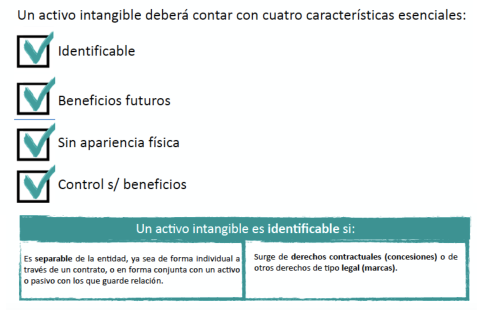
\includegraphics[width=6cm]{\rutaImagenes/def_act_int}\\

\caption{Valor de la Firma \label{fig:valor_firma}}
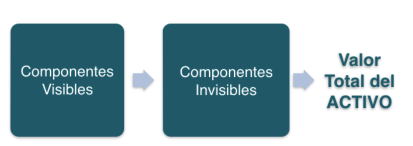
\includegraphics[width=6cm]{\rutaImagenes/valor_firma}
\end{figure}